\documentclass[12pt,addpoints]{repaso}
\grado{1}
\nivel{Secundaria}
\cicloescolar{2024-2025}
\materia{Matemáticas 1 \normalfont \color{darkgray} \\[-0.2em] \small con adecuación curricular a Matemáticas 1$^\circ$ de Primaria.}
\unidad{1, 2 y 3}
\title{Practica la Unidad}
\aprendizajes{\scriptsize%
\item Expresa oralmente la sucesión numérica hasta cuatro cifras, en español y hasta donde sea posible, en su lengua materna, de manera ascendente y descendente a partir de un número natural dado.\\[-1.8em]
\item Representa, con apoyo de material concreto y modelos gráficos, fracciones: medios, cuartos, octavos, dieciseisavos, para expresar el resultado de mediciones y repartos en situaciones vinculadas a su contexto.\\[-1.8em]
\item Resuelve situaciones problemáticas vinculadas a su contexto que implican sumas, restas, multiplicación y división de números naturales de hasta tres cifras utilizando el algoritmo convencional y que impliquen, medición, estimación y comparación, de longitudes, masas y capacidades, con el uso del metro, kilogramo, litro y medios y cuartos de estas unidades; en el caso de la longitud, el decímetro y centímetro.\\[-1.8em]
   }
\author{Melchor Pinto, JC}
\begin{document}
\INFO%
% \begin{multicols}{2}
\tableofcontents
% \end{multicols}
\newpage
\begin{questions}\large
	\addcontentsline{toc}{section}{Unidad 1}
	\section*{Unidad 1}

	\addcontentsline{toc}{subsection}{Conteo de números}
	\subsection*{Conteo de números}

	\questionboxed[15]{Escribe sobre la línea la cantidad de puntos {\color{red} rojos} que aparecen en cada figura:

		\begin{multicols}{5}
			\begin{parts}
				\part 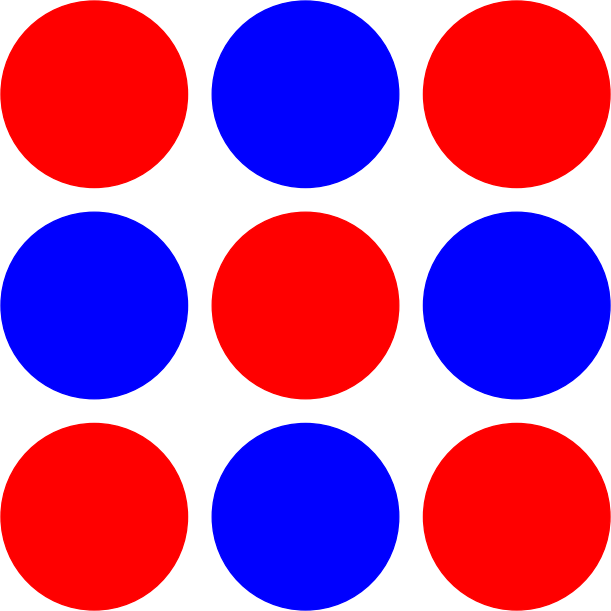
\includegraphics[width=45px]{../images/imagen_puntos01.png} \fillin[ 5][1.5cm]
				\part 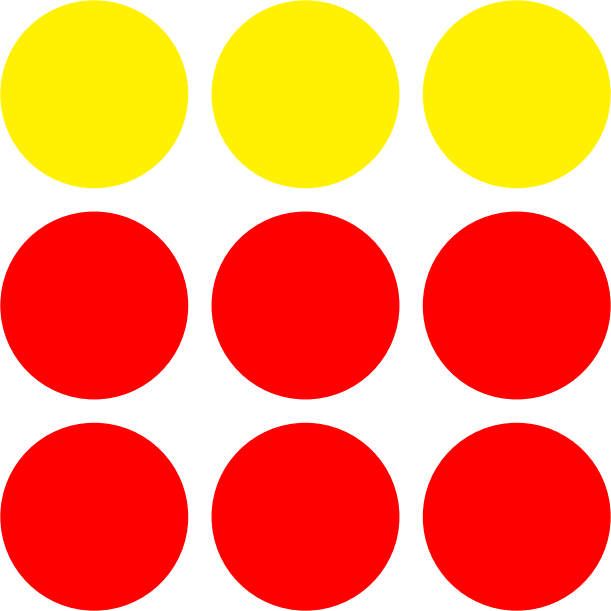
\includegraphics[width=45px]{../images/imagen_puntos05.png} \fillin[ 6][1.5cm]
				\part 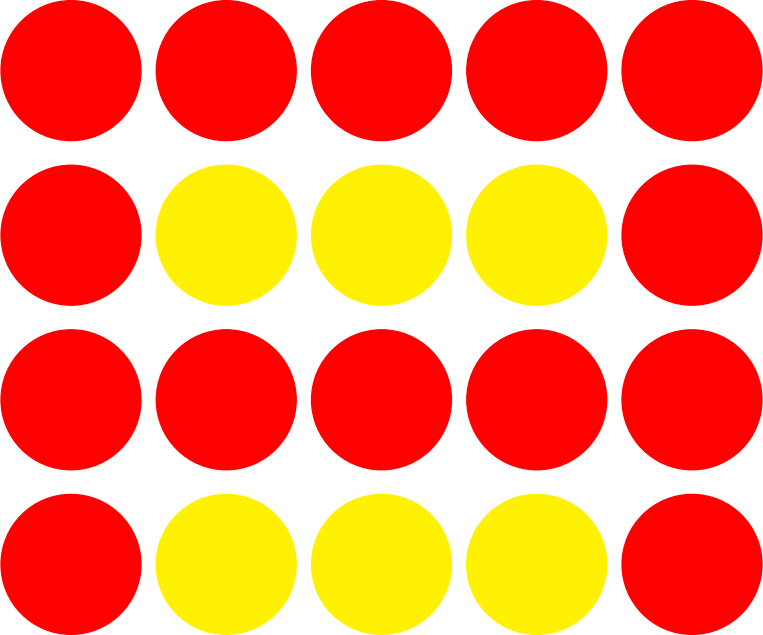
\includegraphics[width=45px]{../images/imagen_puntos09.png} \fillin[14][1.5cm]
				\part 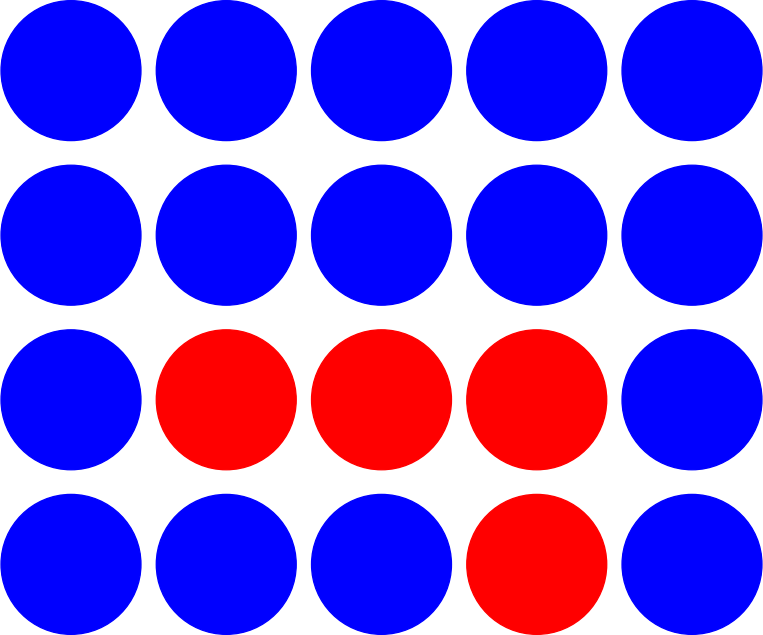
\includegraphics[width=45px]{../images/imagen_puntos13.png} \fillin[ 4][1.5cm]
				\part 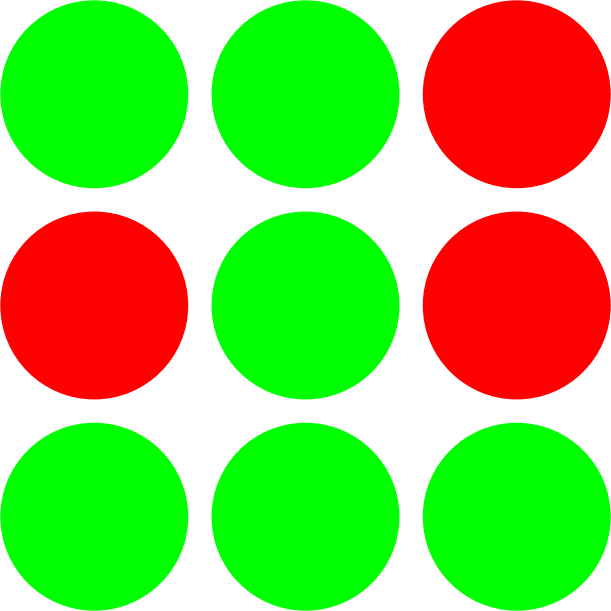
\includegraphics[width=45px]{../images/imagen_puntos02.png} \fillin[ 3][1.5cm]
				\part 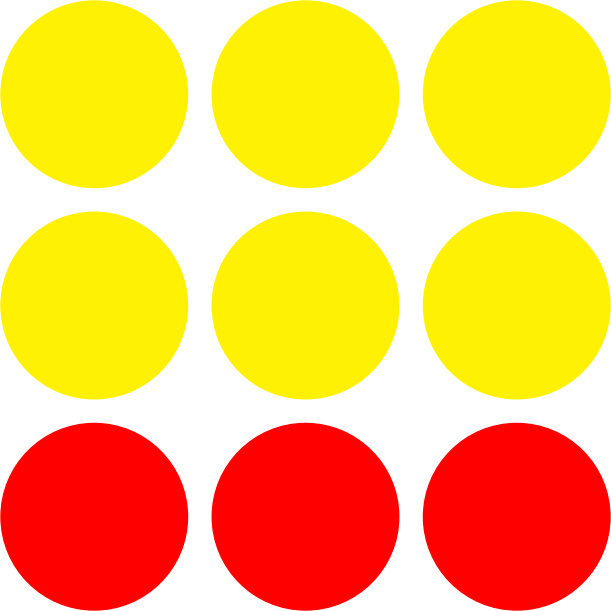
\includegraphics[width=45px]{../images/imagen_puntos06.png} \fillin[ 3][1.5cm]
				\part 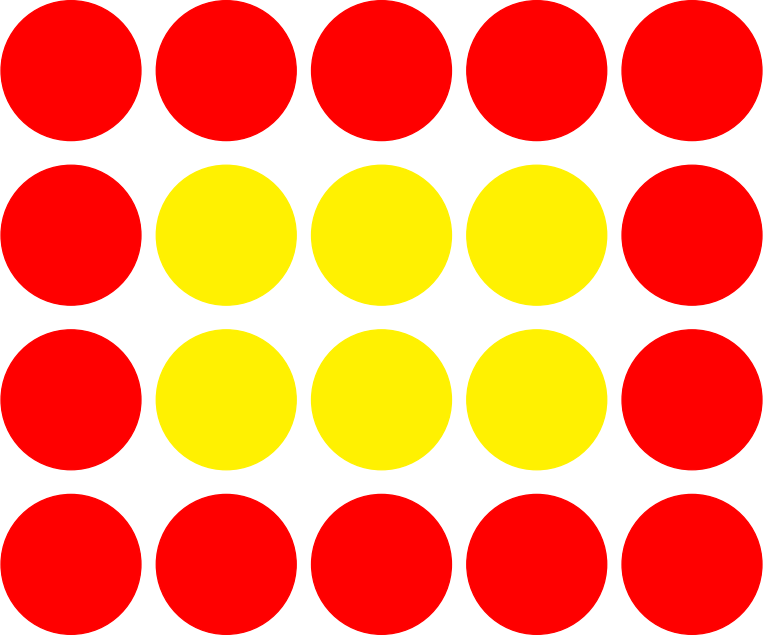
\includegraphics[width=45px]{../images/imagen_puntos10.png} \fillin[14][1.5cm]
				\part 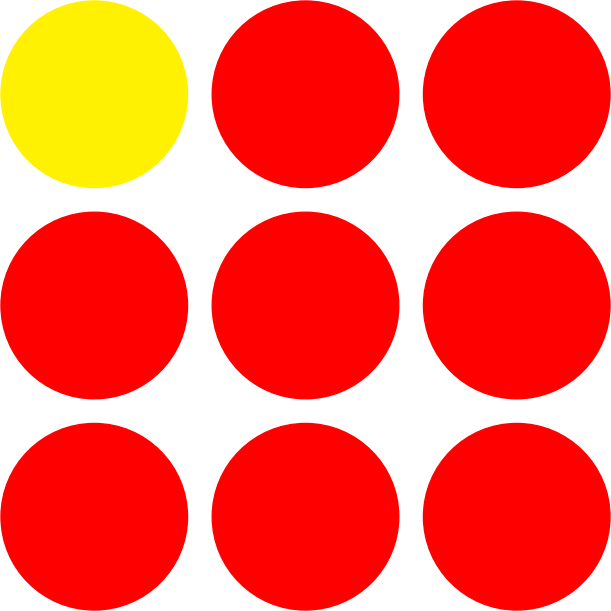
\includegraphics[width=45px]{../images/imagen_puntos07.png} \fillin[ 8][1.5cm]
				\part 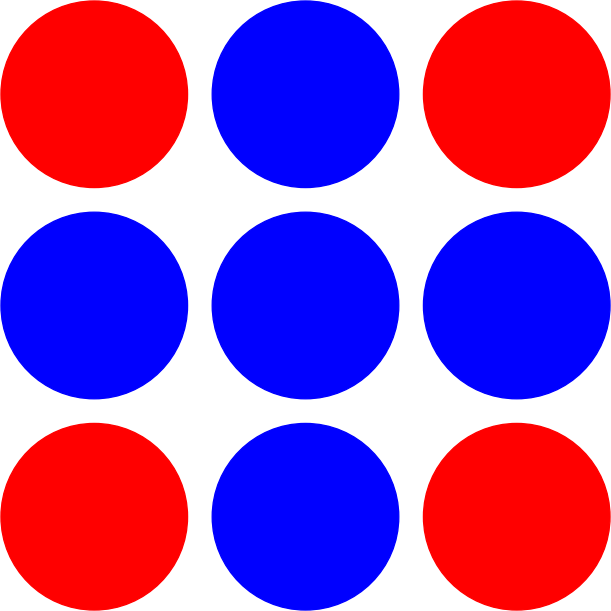
\includegraphics[width=45px]{../images/imagen_puntos03.png} \fillin[ 4][1.5cm]
				\part 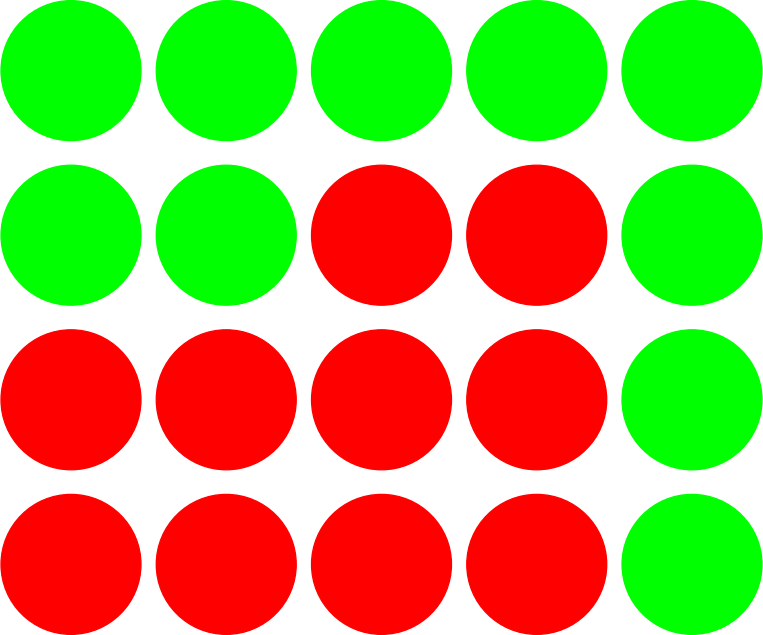
\includegraphics[width=45px]{../images/imagen_puntos14.png} \fillin[10][1.5cm]
				\part 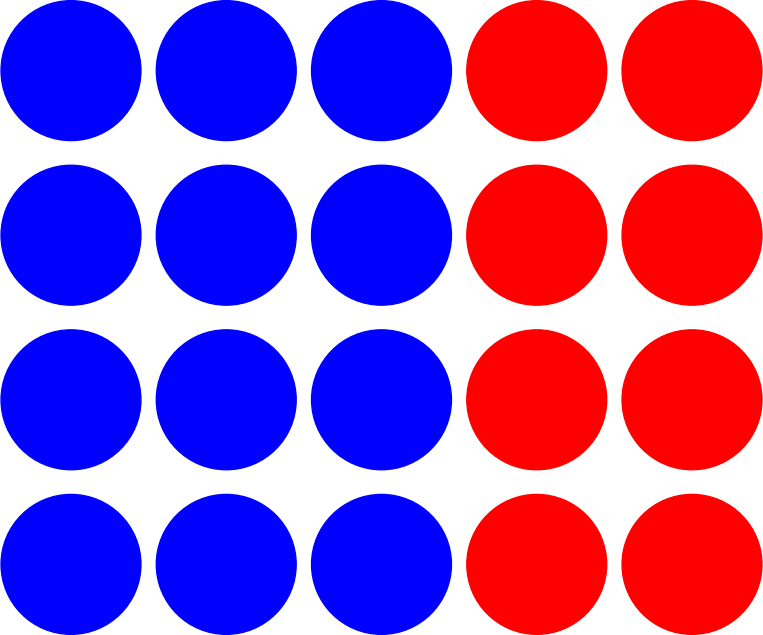
\includegraphics[width=45px]{../images/imagen_puntos11.png} \fillin[ 8][1.5cm]
				\part 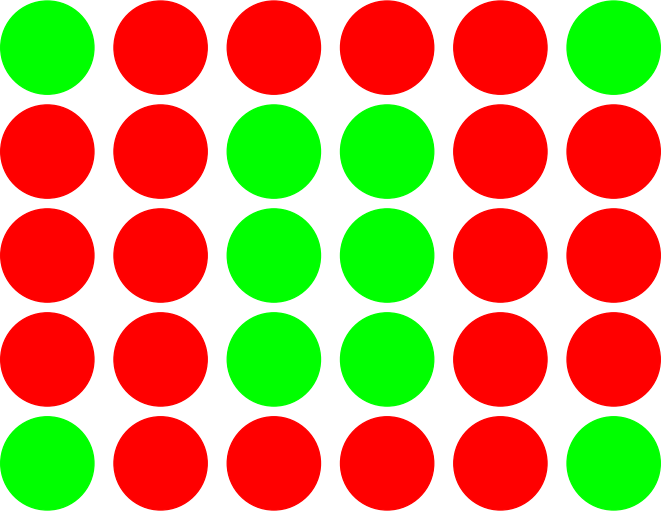
\includegraphics[width=45px]{../images/imagen_puntos15.png} \fillin[20][1.5cm]
				% \part 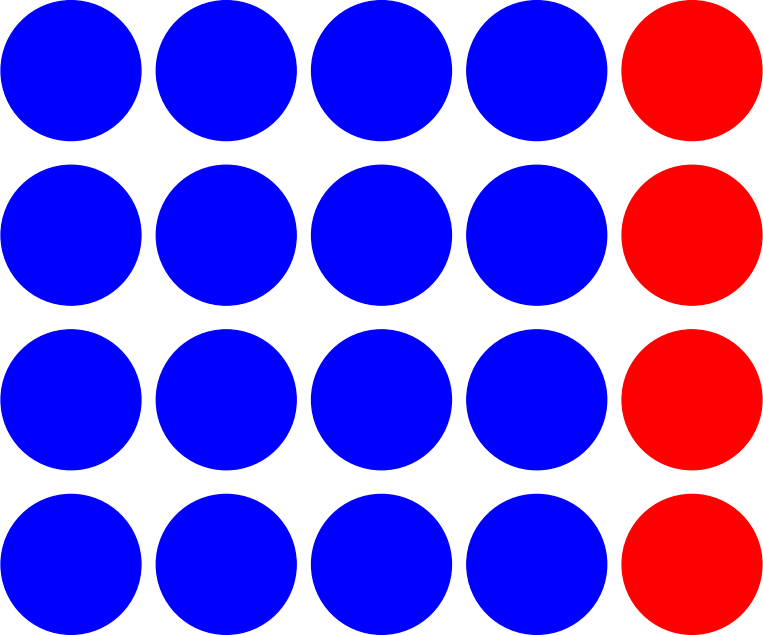
\includegraphics[width=45px]{../images/imagen_puntos12.png} \fillin[ 4][1.5cm] 
				\part 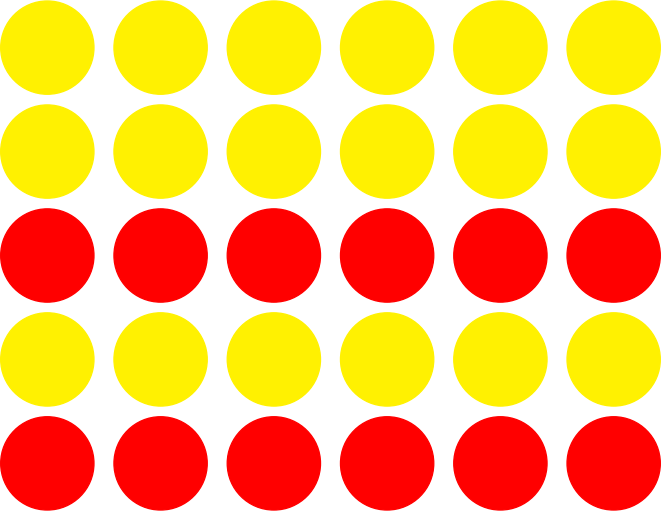
\includegraphics[width=45px]{../images/imagen_puntos16.png} \fillin[10][1.5cm]
				\part 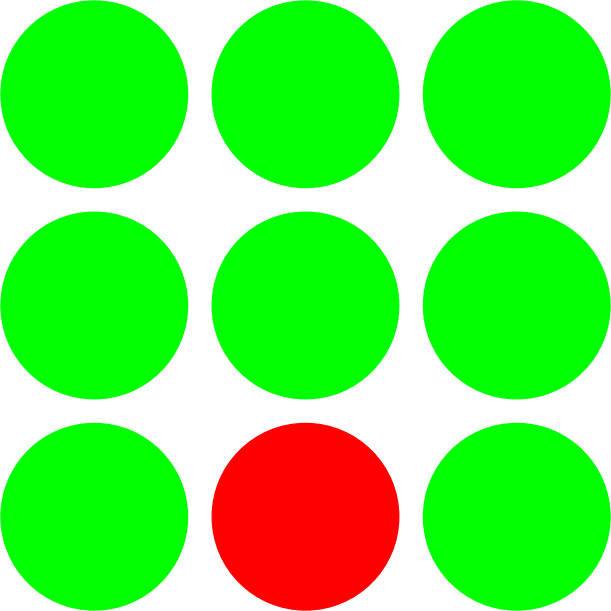
\includegraphics[width=45px]{../images/imagen_puntos04.png} \fillin[ 1][1.5cm]
				\part 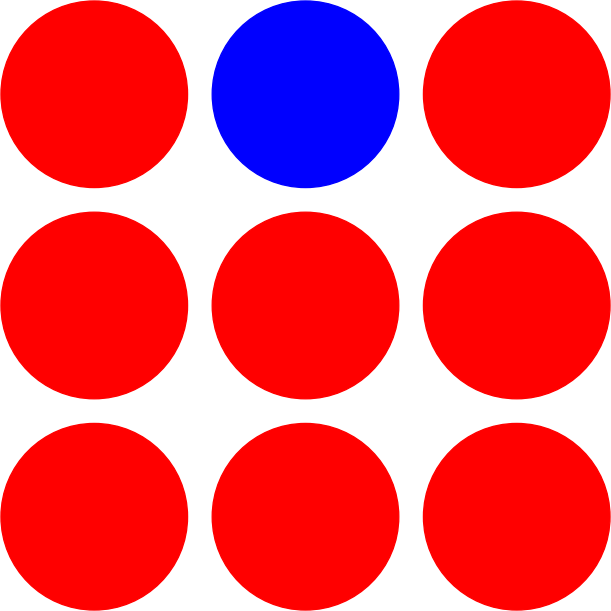
\includegraphics[width=45px]{../images/imagen_puntos08.png} \fillin[ 8][1.5cm]
			\end{parts}
		\end{multicols}
	}

	% \questionboxed[5]{Escribe sobre la línea la cantidad de puntos {\color{red} rojos} que aparecen en cada figura:

	% 	\begin{multicols}{5}
	% 		\begin{parts}
	% 			\part 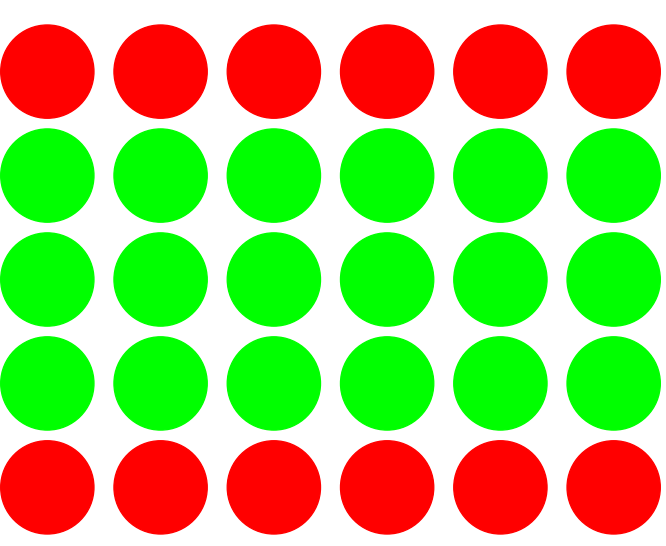
\includegraphics[width=45px]{../images/imagen_puntos17.png} \fillin[12][1.5cm]
	% 			\part 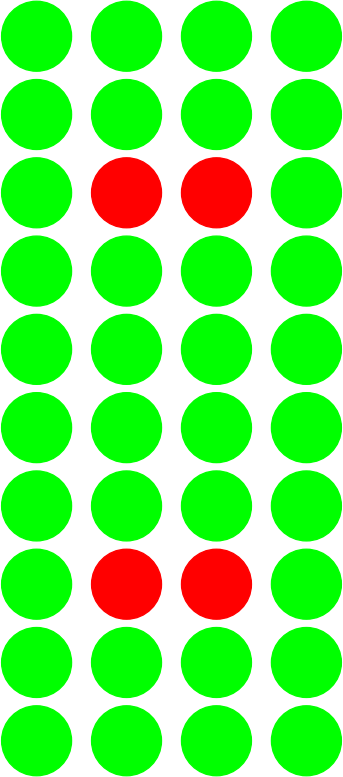
\includegraphics[width=45px]{../images/imagen_puntos25.png} \fillin[ 4][1.5cm]
	% 			\part 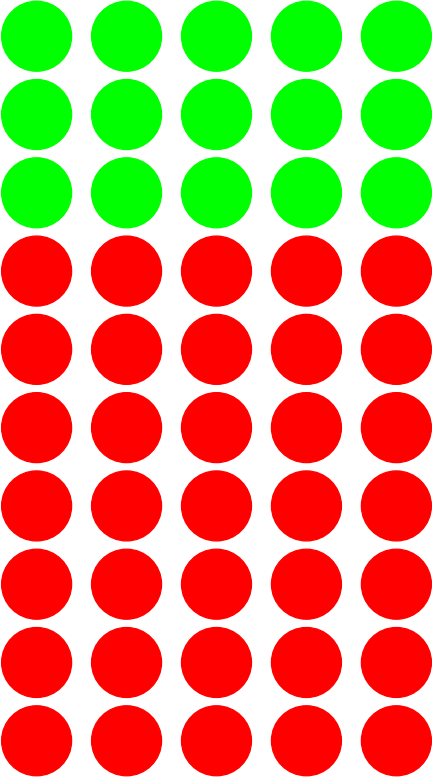
\includegraphics[width=45px]{../images/imagen_puntos29.png} \fillin[35][1.5cm]
	% 			\part 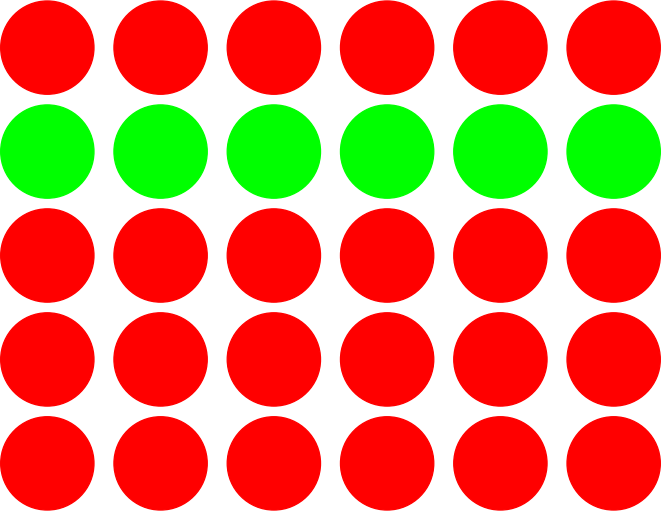
\includegraphics[width=45px]{../images/imagen_puntos21.png} \fillin[24][1.5cm]
	% 			\part 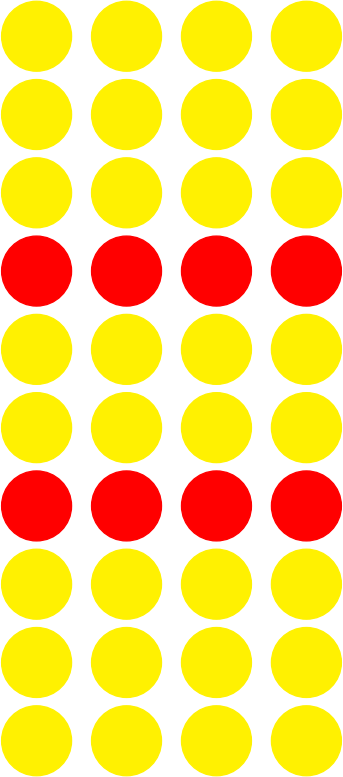
\includegraphics[width=45px]{../images/imagen_puntos22.png} \fillin[ 8][1.5cm]
	% 			\part 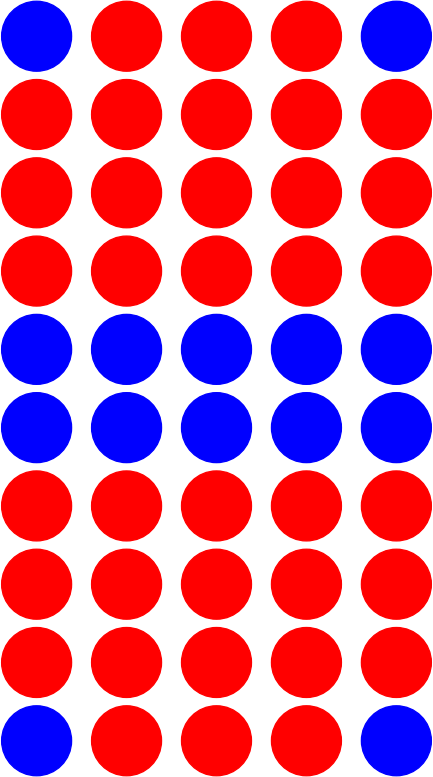
\includegraphics[width=45px]{../images/imagen_puntos30.png} \fillin[36][1.5cm]
	% 			\part 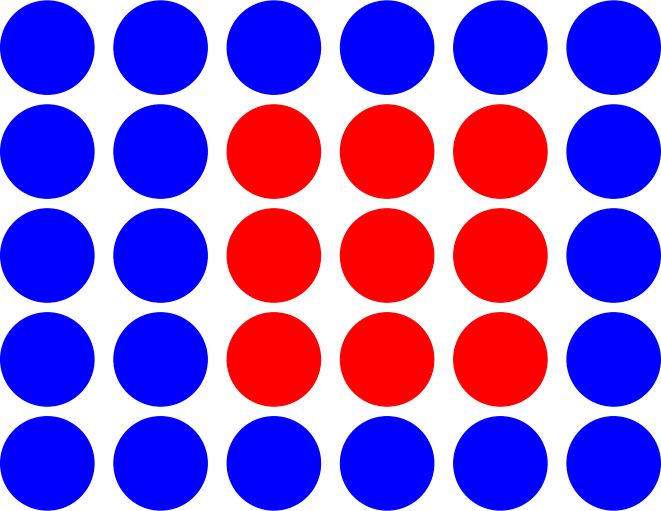
\includegraphics[width=45px]{../images/imagen_puntos18.png} \fillin[ 9][1.5cm]
	% 			\part 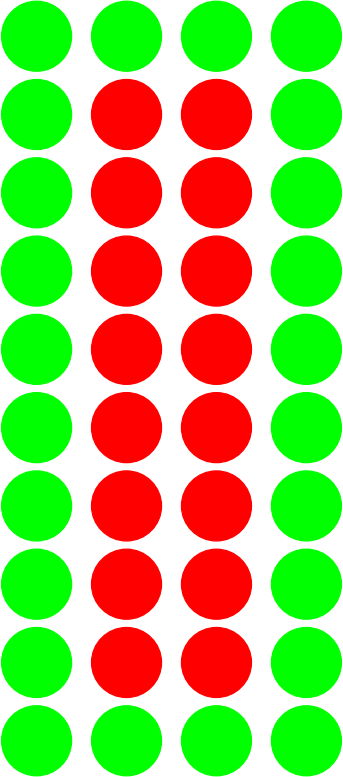
\includegraphics[width=45px]{../images/imagen_puntos26.png} \fillin[16][1.5cm]
	% 			\part 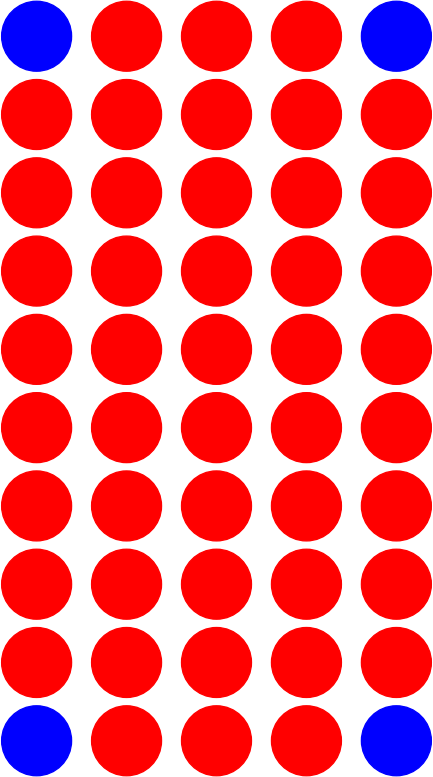
\includegraphics[width=45px]{../images/imagen_puntos31.png} \fillin[46][1.5cm]
	% 			\part 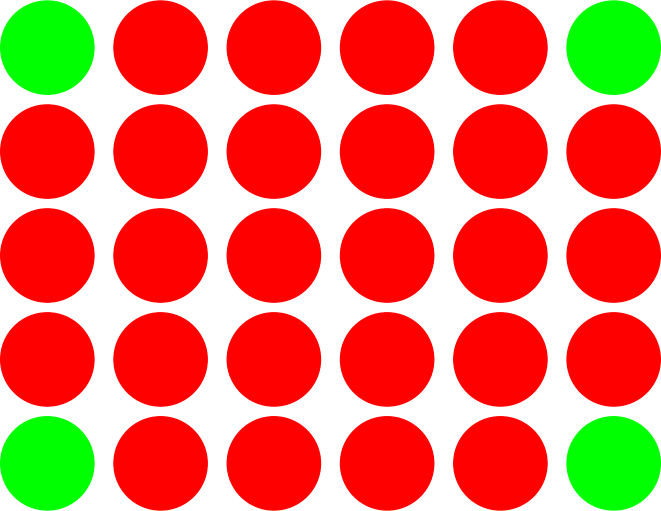
\includegraphics[width=45px]{../images/imagen_puntos19.png} \fillin[26][1.5cm]
	% 			\part 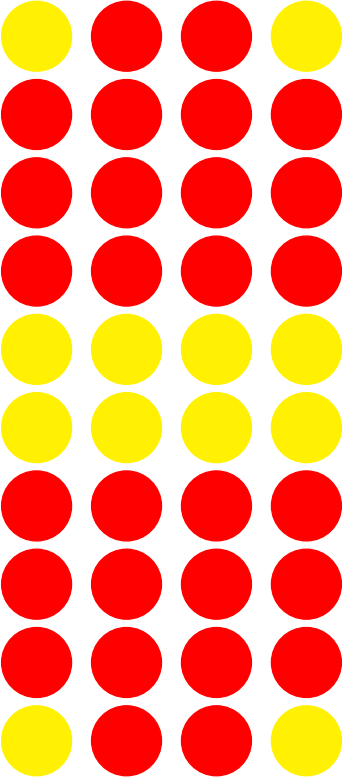
\includegraphics[width=45px]{../images/imagen_puntos23.png} \fillin[28][1.5cm]
	% 			\part 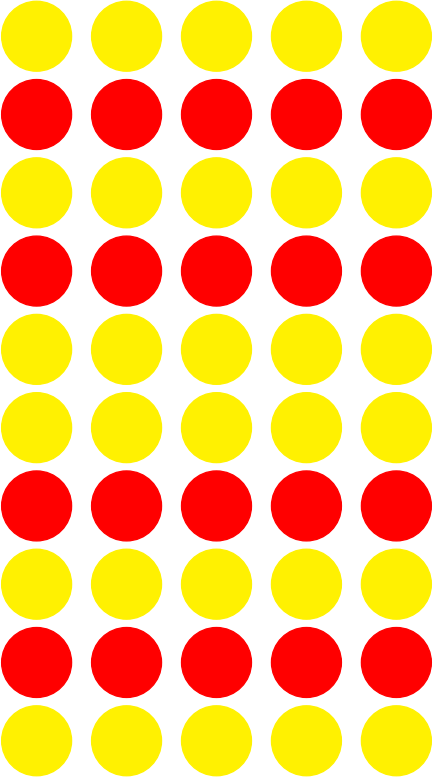
\includegraphics[width=45px]{../images/imagen_puntos28.png} \fillin[20][1.5cm]
	% 			% \part 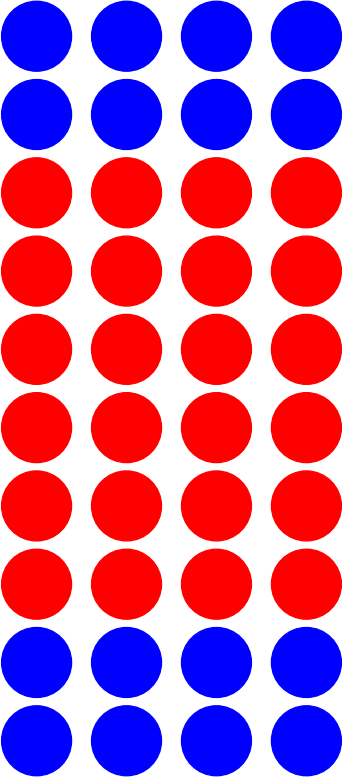
\includegraphics[width=45px]{../images/imagen_puntos27.png} \fillin[24][1.5cm] 
	% 			\part 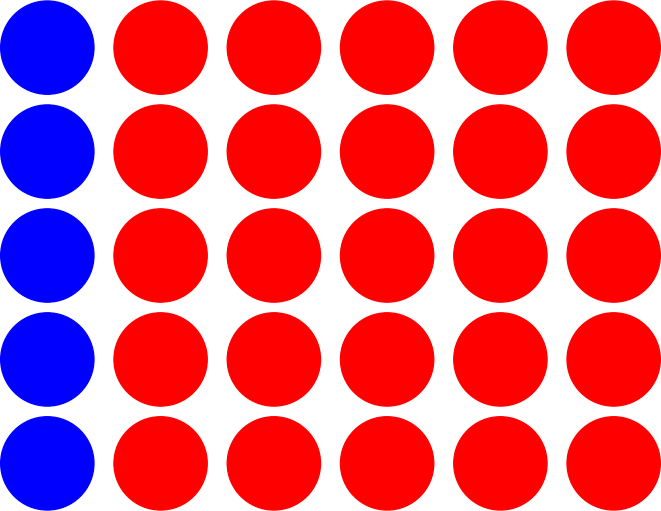
\includegraphics[width=45px]{../images/imagen_puntos20.png} \fillin[25][1.5cm]
	% 			\part 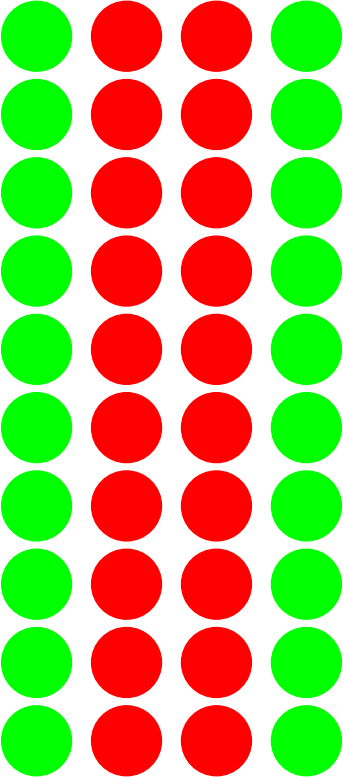
\includegraphics[width=45px]{../images/imagen_puntos24.png} \fillin[20][1.5cm]
	% 			\part 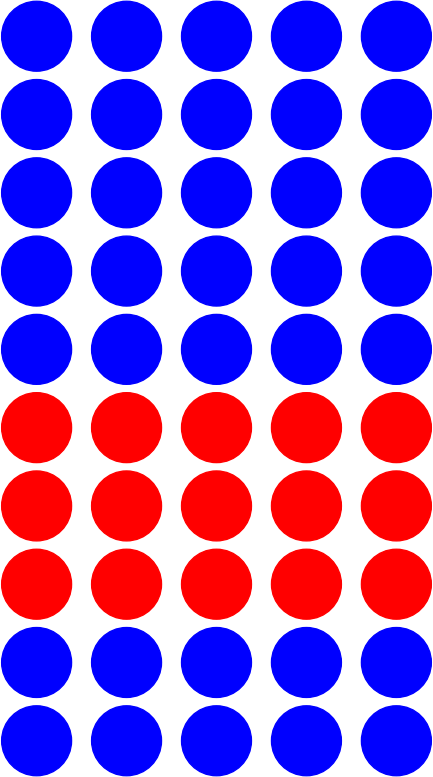
\includegraphics[width=45px]{../images/imagen_puntos32.png} \fillin[15][1.5cm]
	% 		\end{parts}
	% 	\end{multicols}
	% }


	\addcontentsline{toc}{subsection}{Recta numérica}
	\subsection*{Recta numérica}

	\questionboxed[10]{Escribe en el recuadro el número que representa el punto en la recta numérica de cada imagen:

		\begin{multicols}{2}
			\begin{parts}
				\part 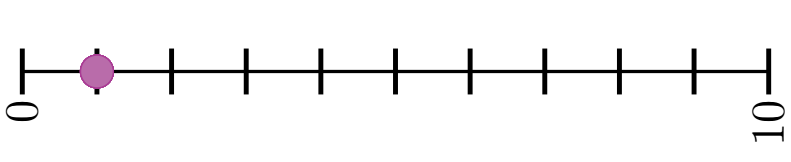
\includegraphics[width=180px]{../images/recta_num_1.png}   \hfill \fillin[ 1][1cm]
				\part 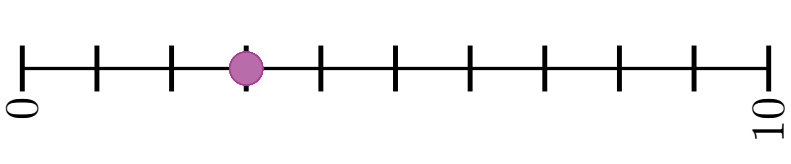
\includegraphics[width=180px]{../images/recta_num_3.png}   \hfill \fillin[ 3][1cm]
				\part 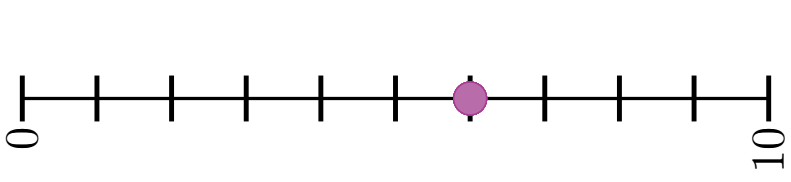
\includegraphics[width=180px]{../images/recta_num_6.png}   \hfill \fillin[ 6][1cm]
				\part 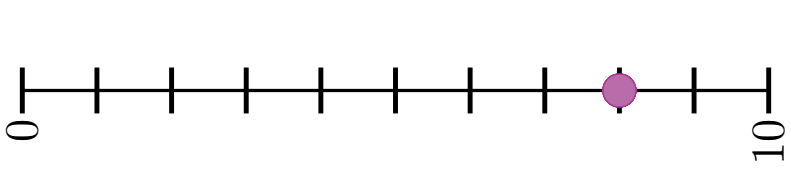
\includegraphics[width=180px]{../images/recta_num_8.png}   \hfill \fillin[ 8][1cm]
				\part 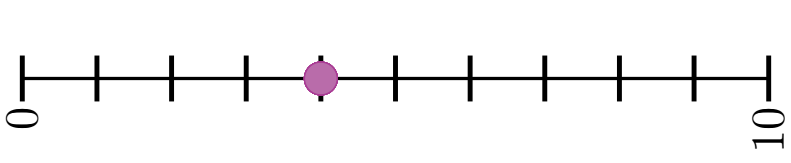
\includegraphics[width=180px]{../images/recta_num_4.png}   \hfill \fillin[ 4][1cm]
				\part 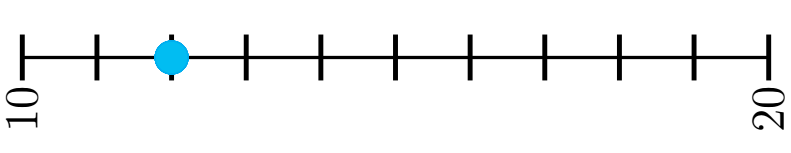
\includegraphics[width=180px]{../images/recta_num_12.png}  \hfill \fillin[12][1cm]
				\part 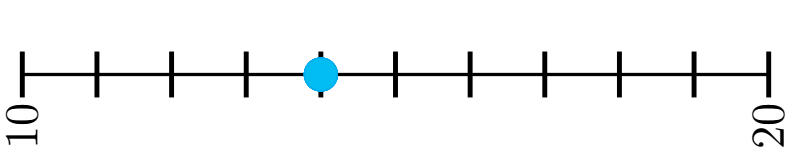
\includegraphics[width=180px]{../images/recta_num_14.png}  \hfill \fillin[14][1cm]
				\part 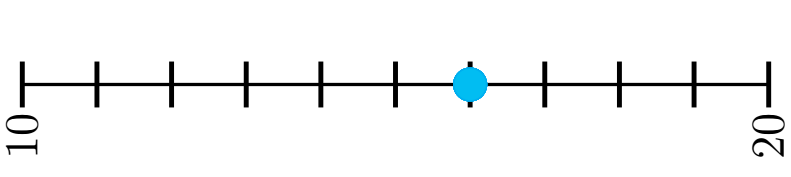
\includegraphics[width=180px]{../images/recta_num_16.png}  \hfill \fillin[16][1cm]
				\part 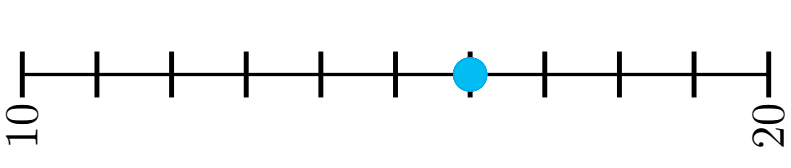
\includegraphics[width=180px]{../images/recta_num_17.png}  \hfill \fillin[17][1cm]
				\part 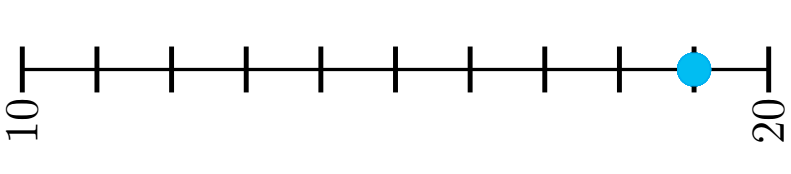
\includegraphics[width=180px]{../images/recta_num_19.png}  \hfill \fillin[19][1cm]
			\end{parts}
		\end{multicols}
	}

	\addcontentsline{toc}{subsection}{Escritura de cantidades}
	\subsection*{Escritura de cantidades}


	\questionboxed[15]{Escribe sobre la línea los siguientes números:

		\begin{multicols}{3}
			\begin{parts}
				\part \fillin[ 2][0.5cm] Dos
				\part \fillin[19][0.5cm] Diecinueve
				\part \fillin[32][0.5cm] Treinta y dos
				\part \fillin[16][0.5cm] Dieciséis
				\part \fillin[21][0.5cm] Veintiuno
				% \part \fillin[67][0.5cm] Sesenta y siete
				% \part \fillin[51][0.5cm] Cincuenta y uno


				\part \fillin[ 5][0.5cm] Cinco
				\part \fillin[43][0.5cm] Cuarenta y tres
				\part \fillin[11][0.5cm] Once
				\part \fillin[18][0.5cm] Dieciocho
				\part \fillin[22][0.5cm] Veintidos
				% \part \fillin[89][0.5cm] Ochenta y nueve
				% % \part \fillin[][0.5cm] Veintinueve
				% \part \fillin[76][0.5cm] Setenta y seis

				\part \fillin[ 9][0.5cm] Nueve
				\part \fillin[13][0.5cm] Trece
				\part \fillin[15][0.5cm] Quince
				\part \fillin[12][0.5cm] Doce
				\part \fillin[27][0.5cm] Veintisiete
				% \part \fillin[60][0.5cm] Sesenta
				% \part \fillin[75][0.5cm] Setenta y cinco
			\end{parts}
		\end{multicols}
	}



	% \questionboxed[5]{Escribe en el recuadro el número que representa el punto en la recta numérica de cada imagen:

	% 	\begin{multicols}{2}
	% 		\begin{parts}
	% 			\part 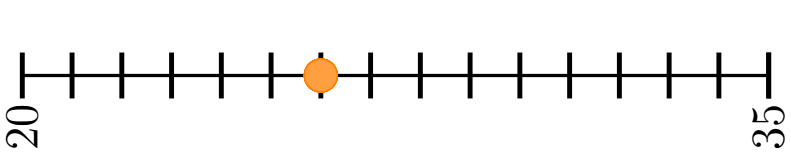
\includegraphics[width=180px]{../images/recta_num_26.png}   \hfill \fillin[26][1cm]
	% 			\part 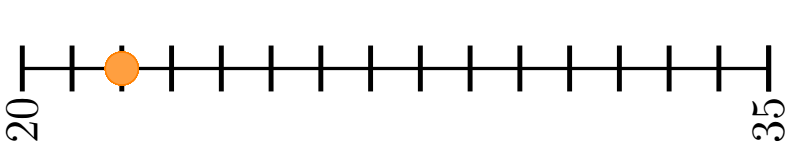
\includegraphics[width=180px]{../images/recta_num_21.png}   \hfill \fillin[21][1cm]
	% 			\part 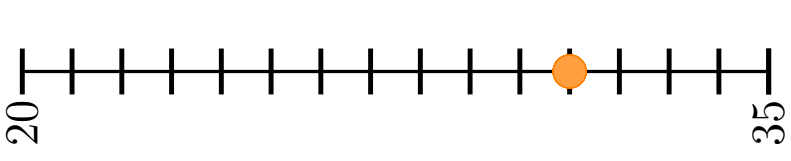
\includegraphics[width=180px]{../images/recta_num_31.png}   \hfill \fillin[31][1cm]
	% 			\part 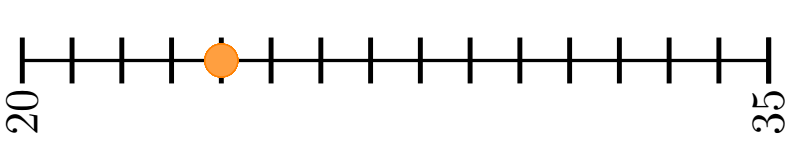
\includegraphics[width=180px]{../images/recta_num_24.png}   \hfill \fillin[24][1cm]
	% 			\part 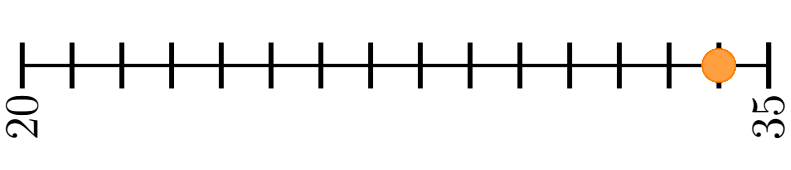
\includegraphics[width=180px]{../images/recta_num_34.png}   \hfill \fillin[34][1cm]
	% 			\part 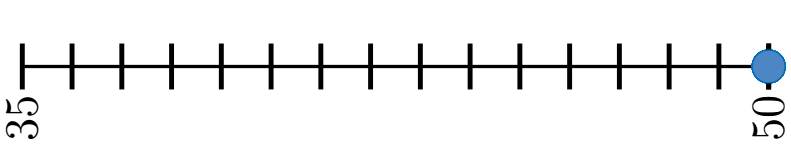
\includegraphics[width=180px]{../images/recta_num_50.png}   \hfill \fillin[50][1cm]
	% 			\part 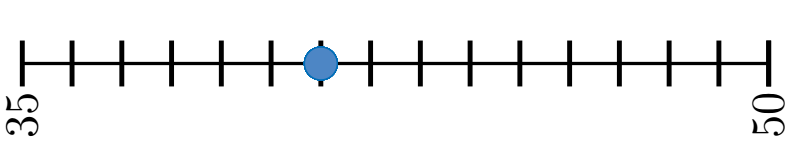
\includegraphics[width=180px]{../images/recta_num_41.png}   \hfill \fillin[41][1cm]
	% 			\part 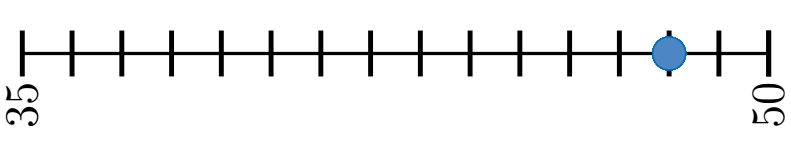
\includegraphics[width=180px]{../images/recta_num_48.png}   \hfill \fillin[48][1cm]
	% 			\part \includegraphics[width=180px]{../images/recta_num_36.png}   \hfill \fillin[36][1cm]
	% 			\part \includegraphics[width=180px]{../images/recta_num_39.png}   \hfill \fillin[39][1cm]
	% 		\end{parts}
	% 	\end{multicols}
	% }

	\addcontentsline{toc}{subsection}{Sistema decimal}
	\subsection*{Sistema decimal}

	\questionboxed[5]{Señala la opción que responda correctamente a cada una de las siguientes preguntas:

		\begin{multicols}{2}
			\begin{parts}
				\part ¿Qué lugar ocupa el 8 en 6418?     \fillin[C][0.5cm]
				\part ¿Qué lugar ocupa el 4 en 206418?   \fillin[A][0.5cm]
				\part ¿Qué lugar ocupa el 6 en 87264?    \fillin[B][0.5cm]
				% \part ¿Qué lugar ocupa el 4 en 1684?     \fillin[C][0.5cm]
				% \part ¿Qué lugar ocupa el 1 en 6138?     \fillin[A][0.5cm]
				% \part ¿Qué lugar ocupa el 4 en 198114?   \fillin[C][0.5cm]
				\part ¿Qué lugar ocupa el 8 en 149778?   \fillin[C][0.5cm]
				\part ¿Qué lugar ocupa el 7 en 46878?    \fillin[B][0.5cm]
			\end{parts}

			\columnbreak%

			\begin{choices}\Large
				\choice {\color{red}centenas.}
				\choice {\color{blue}decenas.}
				\choice {\color{Goldenrod!65!black}unidades.}
			\end{choices}
		\end{multicols}
	}

	\questionboxed[9]{Escribe la notación desarrollada de cada uno de los siguientes números:

		\begin{multicols}{3}
			\begin{parts}
				\part $28=$ \fillin[$20+8$][1in]
				\part $84=$ \fillin[$80+4$][1in]
				\part $77=$ \fillin[$70+7$][1in]
				% \part $936 =$ \fillin[$900+30+6$][1in]

				\part $11 =$ \fillin[$10+1$][1in]
				\part $48 =$ \fillin[$40+8$][1in]
				\part $96=$ \fillin[$90+6$][1in]
				% \part $215 =$ \fillin[$200+10+5$][1in]

				\part $39=$ \fillin[$30+9$][1in]
				\part $57 =$ \fillin[$50+7$][1in]
				\part $79=$ \fillin[$70+9$][1in]
				% \part $105 =$ \fillin[$100+5$][1in]
			\end{parts}
		\end{multicols}
	}

	\newpage
	\addcontentsline{toc}{section}{Unidad 2}
	\section*{Unidad 2}

	\addcontentsline{toc}{subsection}{Sumas}
	\subsection*{Sumas}
	\questionboxed[12]{Realiza las siguientes sumas:

	\begin{multicols}{4}
		\begin{parts}
			\part $9 + 8=$ \fillin[17][0cm]\\[0.2cm]
			\part $5 + 4=$ \fillin[9][0cm]\\[0.2cm]

			\part
			\ifprintanswers{\opadd[hfactor=decimal,resultstyle=\color{red},carryadd=true]{17}{18}}
			\else{\opadd[hfactor=decimal,resultstyle=\color{white},carryadd=false]{17}{18}}\fi\\[0.2cm]

\columnbreak%

			\part $1 + 1=$ \fillin[2][0cm]\\[0.2cm]
			\part $5 + 7=$ \fillin[12][0cm]\\[0.2cm]

			\part
			\ifprintanswers{\opadd[hfactor=decimal,resultstyle=\color{red},carryadd=true]{15}{9}}
			\else{\opadd[hfactor=decimal,resultstyle=\color{white},carryadd=false]{15}{9}}\fi\\[0.2cm]
			
			\columnbreak%
			% \part
			% \ifprintanswers{\opadd[hfactor=decimal,resultstyle=\color{red},carryadd=true]{26}{9}}
			% \else{\opadd[hfactor=decimal,resultstyle=\color{white},carryadd=false]{26}{9}\\[0.5cm]}\fi\\[0.2cm]

			% \part
			% \ifprintanswers{\opadd[hfactor=decimal,resultstyle=\color{red},carryadd=true]{27}{12}}
			% \else{\opadd[hfactor=decimal,resultstyle=\color{white},carryadd=false]{27}{12}}\fi\\[0.2cm]

			\part $0 + 7=$ \fillin[7][0cm]\\[0.2cm]
			\part $8 + 7=$ \fillin[15][0cm]\\[0.2cm]

			\part
			\ifprintanswers{\opadd[hfactor=decimal,resultstyle=\color{red},carryadd=true]{10}{9}}
			\else{\opadd[hfactor=decimal,resultstyle=\color{white},carryadd=false]{10}{9}}\fi\\[0.2cm]
		
			\columnbreak%
			% \part
			% \ifprintanswers{\opadd[hfactor=decimal,resultstyle=\color{red},carryadd=true]{37}{8}}
			% \else{\opadd[hfactor=decimal,resultstyle=\color{white},carryadd=false]{37}{8}\\[0.5cm]}\fi\\[0.2cm]

			% \part
			% \ifprintanswers{\opadd[hfactor=decimal,resultstyle=\color{red},carryadd=true]{48}{14}}
			% \else{\opadd[hfactor=decimal,resultstyle=\color{white},carryadd=false]{48}{14}}\fi\\[0.2cm]

			\part $1 + 9=$ \fillin[10][0cm]\\[0.2cm]
			\part $4 + 9=$ \fillin[13][0cm]\\[0.2cm]

			\part
			\ifprintanswers{\opadd[hfactor=decimal,resultstyle=\color{red},carryadd=true]{21}{19}}
			\else{\opadd[hfactor=decimal,resultstyle=\color{white},carryadd=false]{21}{19}}\fi\\[0.2cm]
			% \part
			% \ifprintanswers{\opadd[hfactor=decimal,resultstyle=\color{red},carryadd=true]{44}{25}}
			% \else{\opadd[hfactor=decimal,resultstyle=\color{white},carryadd=false]{44}{25}\\[0.5cm]}\fi\\[0.2cm]

			% \part
			% \ifprintanswers{\opadd[hfactor=decimal,resultstyle=\color{red},carryadd=true]{82}{38}}
			% \else{\opadd[hfactor=decimal,resultstyle=\color{white},carryadd=false]{82}{38}}\fi\\[0.2cm]
		\end{parts}
	\end{multicols}
}

\addcontentsline{toc}{subsection}{Restas}
\subsection*{Restas}

\questionboxed[12]{Realiza las siguientes restas:

	\begin{multicols}{4}
		\begin{parts}
			\part $9 - 3=$ \fillin[6][0cm]\\[0.2cm]
			% \part $15 - \fillin[8][0.5cm]= 7$\\[0.2cm]

			\part
			\ifprintanswers{\opsub[hfactor=decimal,resultstyle=\color{red},carrysub=true]{17}{6}}
			\else{\opsub[hfactor=decimal,resultstyle=\color{white},carrysub=false]{17}{6}}\fi\\[0.2cm]

			\part
			\ifprintanswers{\opsub[hfactor=decimal,resultstyle=\color{red},carrysub=true]{15}{4}}
			\else{\opsub[hfactor=decimal,resultstyle=\color{white},carrysub=false]{15}{4}}\fi\\[0.2cm]

			% \part
			% \ifprintanswers{\opsub[hfactor=decimal,resultstyle=\color{red},carrysub=true]{34}{22}}
			% \else{\opsub[hfactor=decimal,resultstyle=\color{white},carrysub=false]{34}{22}}\fi\\[0.2cm]

			\part $7 - 4=$ \fillin[3][0cm]\\[0.2cm]
			% \part $12 - \fillin[7][0.5cm]= 5$\\[0.2cm]

			\part
			\ifprintanswers{\opsub[hfactor=decimal,resultstyle=\color{red},carrysub=true]{27}{5}}
			\else{\opsub[hfactor=decimal,resultstyle=\color{white},carrysub=false]{27}{5}}\fi\\[0.2cm]

			\part
			\ifprintanswers{\opsub[hfactor=decimal,resultstyle=\color{red},carrysub=true]{14}{11}}
			\else{\opsub[hfactor=decimal,resultstyle=\color{white},carrysub=false]{14}{11}}\fi\\[0.2cm]

			% \part
			% \ifprintanswers{\opsub[hfactor=decimal,resultstyle=\color{red},carrysub=true]{48}{29}}
			% \else{\opsub[hfactor=decimal,resultstyle=\color{white},carrysub=false]{48}{29}}\fi\\[0.2cm]

			\part $8 - 8=$ \fillin[0][0cm]\\[0.2cm]
			% \part $18 - \fillin[14][0.5cm]= 4$\\[0.2cm]

			\part
			\ifprintanswers{\opsub[hfactor=decimal,resultstyle=\color{red},carrysub=true]{8}{5}}
			\else{\opsub[hfactor=decimal,resultstyle=\color{white},carrysub=false]{8}{5}}\fi\\[0.2cm]

			\part
			\ifprintanswers{\opsub[hfactor=decimal,resultstyle=\color{red},carrysub=true]{16}{9}}
			\else{\opsub[hfactor=decimal,resultstyle=\color{white},carrysub=false]{16}{9}}\fi\\[0.2cm]

			% \part
			% \ifprintanswers{\opsub[hfactor=decimal,resultstyle=\color{red},carrysub=true]{57}{43}}
			% \else{\opsub[hfactor=decimal,resultstyle=\color{white},carrysub=false]{57}{43}}\fi\\[0.2cm]

			\part $11 - 4=$ \fillin[7][0cm]\\[0.2cm]
			% \part $25 - \fillin[20][0.5cm]= 5$\\[0.2cm]

			\part
			\ifprintanswers{\opsub[hfactor=decimal,resultstyle=\color{red},carrysub=true]{17}{5}}
			\else{\opsub[hfactor=decimal,resultstyle=\color{white},carrysub=false]{17}{5}}\fi\\[0.2cm]

			\part
			\ifprintanswers{\opsub[hfactor=decimal,resultstyle=\color{red},carrysub=true]{10}{8}}
			\else{\opsub[hfactor=decimal,resultstyle=\color{white},carrysub=false]{10}{8}}\fi\\[0.2cm]

			% \part
			% \ifprintanswers{\opsub[hfactor=decimal,resultstyle=\color{red},carrysub=true]{63}{18}}
			% \else{\opsub[hfactor=decimal,resultstyle=\color{white},carrysub=false]{63}{18}}\fi\\[0.2cm]
		\end{parts}
	\end{multicols}
}

\newpage

\addcontentsline{toc}{section}{Unidad 3}
\section*{Unidad 3}

\addcontentsline{toc}{subsection}{Tabla del 1}
\subsection*{Tabla del 1}

\questionboxed[2]{Contando de \textbf{1 en 1}, contesta las siguientes preguntas:

		\begin{multicols}{3}
			\begin{parts}\normalsize
				\part ¿qué número sigue del 12? \fillin[13][0.7cm]
				\part ¿qué número sigue del 8? \fillin[9][0.7cm]
				% \part ¿qué número sigue del 56? \fillin[60][0.7cm]
				\part ¿qué número sigue del 20? \fillin[21][0.7cm]
				% \part ¿qué número sigue del 18? \fillin[22][0.7cm]
				\part ¿qué número sigue del 6? \fillin[7][0.7cm]
				% \part ¿qué número sigue del 0?  \fillin[ 4][0.7cm]
				\part ¿qué número sigue del 18 ? \fillin[19][0.7cm]
				\part ¿qué número sigue del 2? \fillin[3][0.7cm]
				% \part ¿qué número sigue del 32? \fillin[36][0.7cm]
			\end{parts}
		\end{multicols}
	}

	\addcontentsline{toc}{subsection}{Tabla del 2}
	\subsection*{Tabla del 2}

	\questionboxed[2]{Contando de \textbf{2 en 2}, contesta las siguientes preguntas:

		\begin{multicols}{3}
			\begin{parts}\normalsize
				\part ¿qué número sigue del 15? \fillin[17][0.7cm]
				% \part ¿qué número sigue del 28? \fillin[33][0.7cm]
				% \part ¿qué número sigue del 56? \fillin[61][0.7cm]
				\part ¿qué número sigue del 20? \fillin[22][0.7cm]
				\part ¿qué número sigue del 18? \fillin[20][0.7cm]
				\part ¿qué número sigue del 16? \fillin[18][0.7cm]
				\part ¿qué número sigue del 3?  \fillin[ 5][0.7cm]
				% \part ¿qué número sigue del 7 ? \fillin[12][0.7cm]
				\part ¿qué número sigue del 21? \fillin[26][0.7cm]
				% \part ¿qué número sigue del 32? \fillin[37][0.7cm]
			\end{parts}
		\end{multicols}
	}

	\addcontentsline{toc}{subsection}{Tabla del 3}
	\subsection*{Tabla del 3}

	\questionboxed[2]{Contando de \textbf{3 en 3}, contesta las siguientes preguntas:

		\begin{multicols}{3}
			\begin{parts}\normalsize
				\part ¿qué número sigue del 2? \fillin[5][0.7cm]
				\part ¿qué número sigue del 8? \fillin[11][0.7cm]
				% \part ¿qué número sigue del 56? \fillin[62][0.7cm]
				\part ¿qué número sigue del 10? \fillin[13][0.7cm]
				\part ¿qué número sigue del 16? \fillin[19][0.7cm]
				% \part ¿qué número sigue del 34? \fillin[40][0.7cm]
				\part ¿qué número sigue del 0 ? \fillin[ 3][0.7cm]
				\part ¿qué número sigue del 6 ? \fillin[9][0.7cm]
				% \part ¿qué número sigue del 19? \fillin[25][0.7cm]
				% \part ¿qué número sigue del 30? \fillin[36][0.7cm]
			\end{parts}
		\end{multicols}
	}

	% \questionboxed[12]{Reponde las siguientes tablas de multiplicar:

	% 	\begin{multicols}{4}
	% 		\begin{parts}
	% 			\part $5 \times 9=$ \fillin[45][0.5cm]  
	% 			\part $\fillin[6][0.5cm] \times 4= 24$  
	% 			\part $5 \times 3=$ \fillin[15][0.5cm]  
	% 			\part $5 \times \fillin[10][0.5cm]=50$  
	% 			\part $3 \times 8=$ \fillin[24][0.5cm]  
	% 			\part $4 \times \fillin[8][0.5cm]=32$  
	% 			\part $6 \times 9=$ \fillin[54][0.5cm]  
	% 			\part $4 \times \fillin[5][0.5cm]= 20$  
	% 			\part $3 \times 6=$ \fillin[18][0.5cm]  
	% 			\part $\fillin[2][0.5cm] \times 4= 8$  
	% 			\part $2 \times 7=$ \fillin[14][0.5cm]  
	% 			\part $4 \times \fillin[4][0.5cm]= 16$  
	% 			\part $4 \times 7=$ \fillin[28][0.5cm]  
	% 			\part $\fillin[3][0.5cm] \times 4= 12$  
	% 			\part $3 \times 8=$ \fillin[24][0.5cm]  
	% 			\part $4 \times \fillin[11][0.5cm]= 44$  
	% 			\part $2 \times 9=$ \fillin[18][0.5cm]  
	% 			\part $\fillin[9][0.5cm] \times 5= 45$  
	% 			\part $4 \times 4=$ \fillin[16][0.5cm]  
	% 			\part $4 \times \fillin[9][0.5cm]= 36$  
	% 			\part $10 \times 3=$ \fillin[30][0.5cm]  
	% 			\part $\fillin[7][0.5cm] \times 4= 28$  
	% 			\part $7 \times 6=$ \fillin[42][0.5cm]  
	% 			\part $\fillin[9][0.5cm] \times 3= 27$  
	% 		\end{parts}
	% 	\end{multicols}
	% }


	\addcontentsline{toc}{subsection}{Miselánea}
	\subsection*{Miselánea}

	\questionboxed[6]{Escribe sobre la línea el nombre que recibe cada figura geométrica de acuerdo con su número de lados:

		\begin{multicols}{3}
			\begin{parts}
				\part \includegraphics[width=75px]{../images/pentagono_azul.png}  \fillin[pentágono][0.75in]
				\part \includegraphics[width=75px]{../images/rombo_azul.png}   \fillin[rombo][0.75in]
				\part \includegraphics[width=75px]{../images/circulo_azul.png}   \fillin[círculo][0.75in]
				\part \includegraphics[width=75px]{../images/trapecio_azul.png}   \fillin[trapecio][0.75in]
				\part \includegraphics[width=75px]{../images/rectangulo_azul.png} \fillin[rectángulo][0.75in]
				\part \includegraphics[width=75px]{../images/cuadrado_azul.png}   \fillin[cuadrado][0.75in]
			\end{parts}
		\end{multicols}
	}

	\questionboxed[4]{Clasifica las siguientes fracciones en propias, impropias o mixtas:

		\begin{multicols}{4}
			\begin{parts}
				\part $\dfrac{5}{6}$   \fillin[Propia][1in]     \\[0.5em]
				\part $5\dfrac{5}{11}$ \fillin[Mixta][1in]      \\[0.5em]
				\part $\dfrac{13}{12}$   \fillin[Impropia][1in] \\[0.5em]
				\part $1\dfrac{2}{15}$  \fillin[Mixta][1in]     \\[0.5em]
				\part $\dfrac{42}{43}$   \fillin[Propia][1in]   \\[0.5em]
				\part $\dfrac{16}{9}$   \fillin[Impropia][1in]  \\[0.5em]
				\part $\dfrac{7}{3}$   \fillin[Impropia][1in]   \\[0.5em]
				\part $3\dfrac{2}{9}$  \fillin[Mixta][1in]      \\[0.5em]
				\part $\dfrac{3}{2}$   \fillin[Impropia][1in]   \\[0.5em]
				\part $1\dfrac{2}{3}$  \fillin[Mixta][1in]      \\[0.5em]
				\part $\dfrac{7}{8}$   \fillin[Propia][1in]     \\[0.5em]
				\part $\dfrac{6}{5}$   \fillin[Impropia][1in]   \\[0.5em]
			\end{parts}
		\end{multicols}
	}

	\questionboxed[6]{Escribe sobre la línea la fracción que representa cada imagen:

		\begin{multicols}{5}
			\begin{parts}
				\part \includegraphics[width=0.7\linewidth]{../images/imagen_frac_2prim_8|10.png}  \fillin[$\sfrac{8}{10}$][0.5cm] \\[-0.5em]
				\part \includegraphics[width=0.7\linewidth]{../images/imagen_frac_2prim_5|8.png}   \fillin[$\sfrac{5}{8}$ ][0.5cm] \\[-0.5em]
				\part \includegraphics[width=0.7\linewidth]{../images/imagen_frac_2prim_4|6.png}   \fillin[$\sfrac{4}{6}$ ][0.5cm] \\[-0.5em]
				\part \includegraphics[width=0.7\linewidth]{../images/imagen_frac_2prim_2|5.png}   \fillin[$\sfrac{2}{5}$ ][0.5cm] \\[-0.5em]
				\part \includegraphics[width=0.7\linewidth]{../images/imagen_frac_2prim_3|4.png}   \fillin[$\sfrac{3}{4}$ ][0.5cm] \\[-0.5em]
				\part \includegraphics[width=0.7\linewidth]{../images/imagen_frac_2prim_6|10.png}  \fillin[$\sfrac{6}{10}$][0.5cm] \\[-0.5em]
				\part \includegraphics[width=0.7\linewidth]{../images/imagen_frac_2prim_4|5.png}   \fillin[$\sfrac{4}{5}$ ][0.5cm] \\[-0.5em]
				\part \includegraphics[width=0.7\linewidth]{../images/imagen_frac_2prim_7|10.png}  \fillin[$\sfrac{7}{10}$][0.5cm] \\[-0.5em]
				\part \includegraphics[width=0.7\linewidth]{../images/imagen_frac_2prim_3|10.png}  \fillin[$\sfrac{3}{10}$][0.5cm] \\[-0.5em]
				\part \includegraphics[width=0.7\linewidth]{../images/imagen_frac_2prim_1|4.png}   \fillin[$\sfrac{1}{4}$ ][0.5cm] \\[-0.5em]
			\end{parts}
		\end{multicols}
	}
\end{questions}
\end{document}